\chapter{Apéndice}\label{ch:Ap}

\section{Demostraciones del texto}
\subsection{Solución de un sistema lineal}
Se anexa la demostración al \textbf{Teorema 1} [\ref{teo:Solgral}]:
\begin{proof}
	Se propone la función general $X(t)=e^{\lambda t}\vec{v}_0$. Entonces derivamos la función con respecto del tiempo
	\begin{align*}
		\dot{X}(t) &= \lambda e^{\lambda t}\vec{v}_0\\
				   &= e^{\lambda t}(\lambda\vec{v}_0)\\
				   &= e^{\lambda t}(A\vec{v}_0)		\\
				   &= A(e^{\lambda t}\vec{v}_0)\\
				   &= AX(t)
	\end{align*}
\end{proof}

\subsection{Solución de la ecuación logística}\label{sec:SolEqLogistica}

La ecuación logística (\ref{eqn:EqLogistica}) es de las pocas ecuaciones no lineales de las que podemos hallar una solución analítica única. A continuación nos adentraremos a hallar dicha solución. Reescribimos la ecuación de la siguiente manera
$$\frac{dN}{dt}=\frac{rN(K-N)}{K}$$
se utiliza la separación de variables para poder resolver la ecuación, re acomodando nos queda como
$$\frac{KdN}{N(K-N)}=rdt\qquad\Longleftrightarrow\qquad \int\frac{KdN}{N(K-N)}=\int rdt$$
El lado izquierdo lo resolvemos por fracciones parciales, se encomienda al lector comprobar que la siguiente igualdad es verdadera
$$\frac{K}{N(N-K)}=\frac{1}{N}+\frac{1}{K-N}$$
entonces las integrales ya resueltas nos quedan de la siguiente manera
\begin{align*}
	\ln N-\ln(K-N)&=rt+c \\
	\ln\left (\frac{N}{K-N}\right ) &= rt+c\\
	\frac{N}{K-N}&=e^{rt+c}\\
	N&=(K-N)Ce^{rt}\\
	N(1+Ce^{rt})&=KCe^{rt}\\
	N(t)&=\frac{KCe^{rt}}{1+Ce^{rt}}
\end{align*}
Resolviendo el problema de condición inicial se establece que para $t=0$ se tiene $N(0)=N_0$, por tanto la constante $C$ nos queda como
$$C=\frac{N_0}{K-N_0}$$
Finalmente reajustando y acomodando términos, la solución de la ecuación logística es:
\begin{equation}\label{eqn:SolEqLogistica}
	N(t)=\frac{KN_0e^{rt}}{(K-N_0)+N_0e^{rt}}
\end{equation}
Comparado con la solución numérica se ve de la siguiente forma
\begin{figure}[h!]
	\centering
	\includegraphics[scale=0.23]{../../Imagenes/Ecuacion Logistica Analítica}
	\caption{Ecuación logística con una tasa de crecimiento $r=2$ y una capacidad de carga $K=10$, se grafica para las mismas condiciones iniciales; (\textbf{A}) Solución analítica. (\textbf{B}) Solución numérica.}
	\label{fig:EcuacionLogisticaAnalitica}
\end{figure}
\newpage
\subsection{Solución del sistema presa-depredador}\label{sec:SolPresaDepredador}

El sistema (\ref{eqn:PresaDepredador}) tiene la dicha de poderse resolver de forma analítica al igual que la ecuación logística y se verá a continuación el procedimiento. Para ello definimos la siguiente regla de la cadena para $y(t)$
$$\frac{dy}{dt} = \frac{dy}{dx}\cdot\frac{dx}{dt}\qquad\Longleftrightarrow\qquad\frac{dy}{dx}=\frac{\frac{dy}{dt}}{\frac{dx}{dt}}$$
sustituyendo las ecuaciones de (\ref{eqn:PresaDepredador}) en $\frac{dy}{dx}$ se tiene
\begin{align*}
	\frac{dy}{dx}&=\frac{\delta xy-\gamma y}{\alpha x-\beta xy}  \\
\end{align*}
Se factoriza lo necesario y se aplica separación de variables para poder integrar las ecuaciones y hallar las soluciones
\begin{align*}
	x(\alpha-\beta y)\, dy &= y(\delta x-\gamma)\, dx\\
	\int \frac{\alpha-\beta y}{y}\, dy &= \int \frac{\delta x-\gamma}{x}\, dx \\
\end{align*}
al integrar finalmente tenemos la solución implícita:
\begin{equation}\label{eqn:CurvasNivelPD}
	f(x,y)=\alpha\ln y+\gamma\ln x-\beta y- \delta x=c
\end{equation}
Ahora veamos las curvas de nivel de la solución analítica en contraste con el espacio fase generado a través de las ecuaciones de (\ref{eqn:PresaDepredador}):
\begin{figure}[h!]
	\centering
	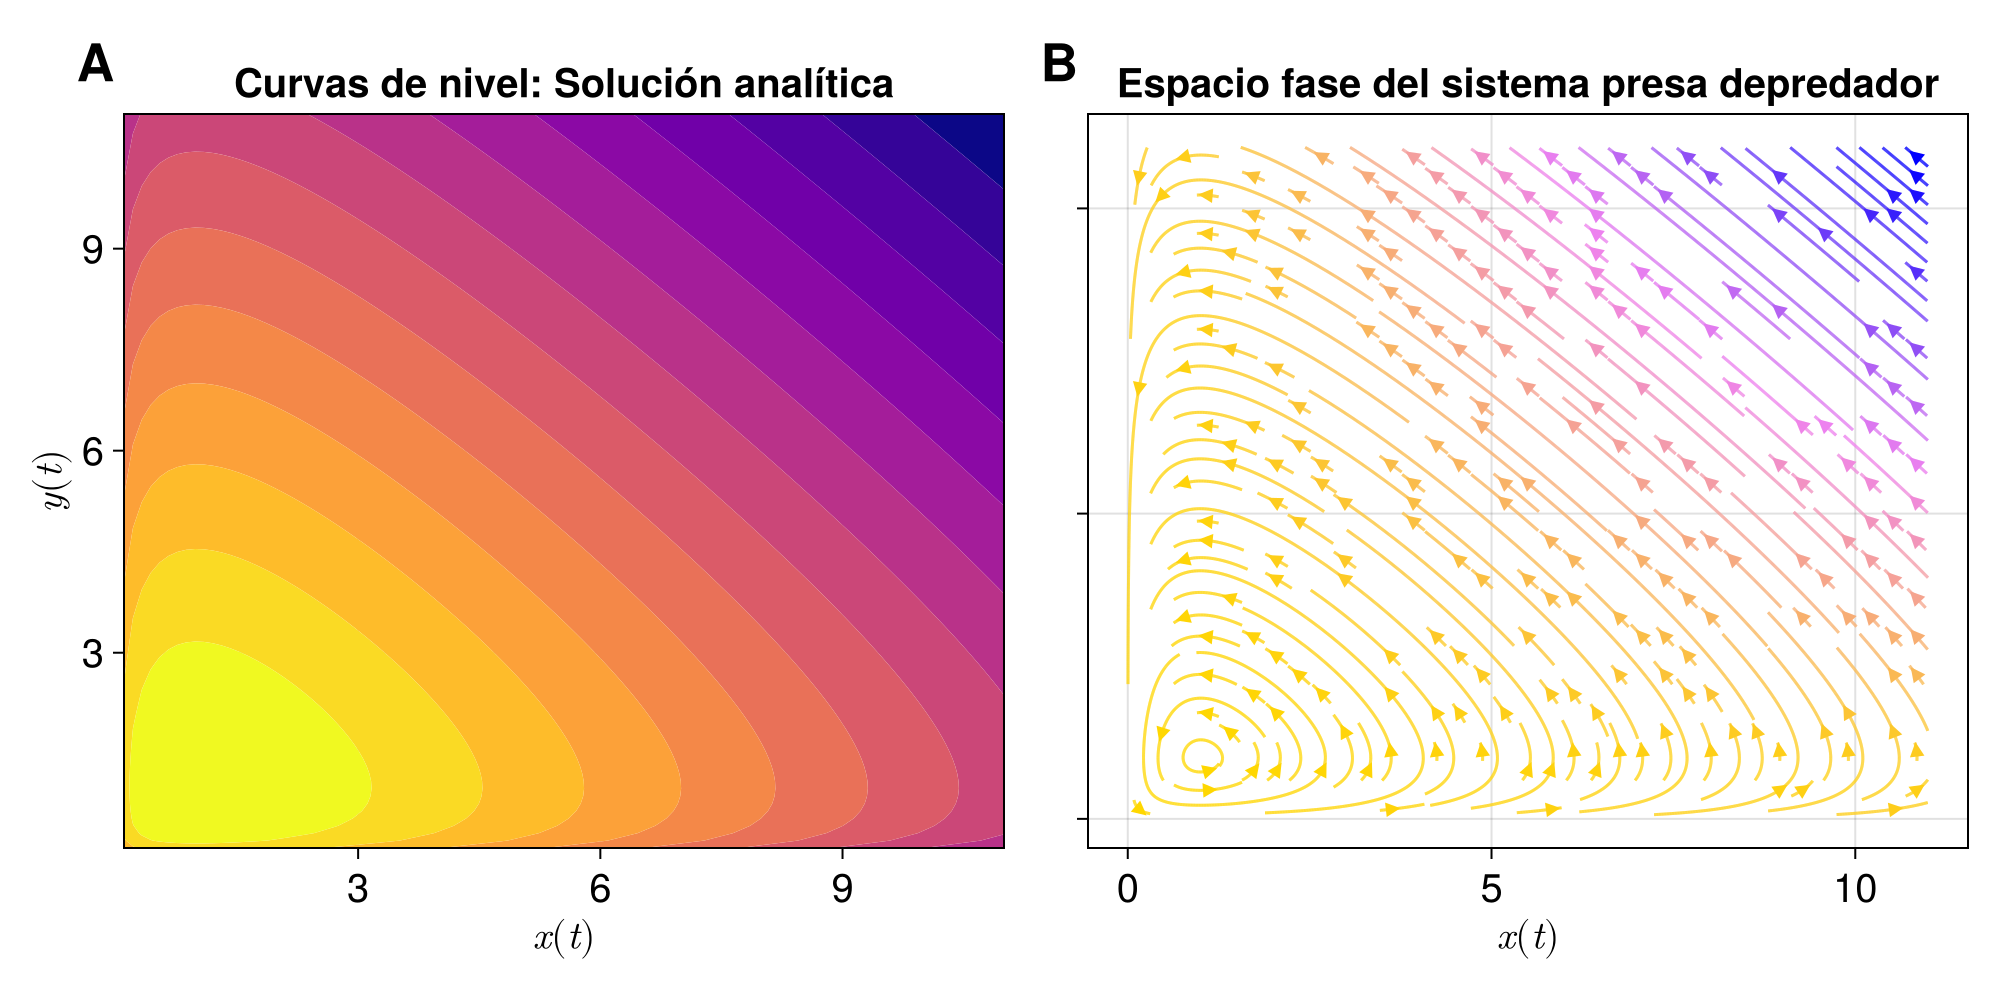
\includegraphics[scale=0.22]{../../Imagenes/Curvas de nivel PD}
	\caption{(\textbf{A}) Curvas de nivel utilizando la solución analítica (\ref{eqn:CurvasNivelPD}). (\textbf{B}) Espacio fase generado a partir de las ecuaciones de (\ref{eqn:PresaDepredador}).}
	\label{fig:CurvasNivelPD}
\end{figure}

\section{Algoritmos y códigos}

El trabajo presente se ha realizado bajo algoritmos, funciones y sintaxis del lenguaje Julia. En esta sección como en otras se estará anexando código en referencia a elementos presentes en el cuerpo de la tesis. Se anexa código de las figuras de los espacios fase de la sección (\ref{sec:Espacios fase}).\\
\\
El bloque de código (\ref{al:EspaciosFase}) funciona para generar la Figura (\ref{fig:EFReales}); sin embargo se puede modificar convenientemente para poder generar las Figuras (\ref{fig:EFComplejos}) y (\ref{fig:CompetenciaEspecies}), únicamente hay que definir las respectivas funciones del sistema para que se pueda generar el campo de direcciones apropiado.
\begin{algorithm}
	\caption{Generación de gráficas de espacios fase de $2\times 2$ con eigenvalores reales usando CairoMakie.}
	\KwData{Matrices de coeficientes.}
	\KwResult{Espacios fase.}
	\label{al:EspaciosFase}
	Inicializar el proceso\;	
	\begin{minted}{julia}
using CairoMakie
xlim = (-3,3)	#Se establecen los límites que abarcarán las gráficas
ylim = (-3,3)

fSilla(X) = Point2(-3X[1],2X[2])  #Se definen las matrices de coeficientes
fAtractor(X) = Point2(-X[1],-4X[2])  #de los sistemas lineales
fRepulsor(X) = Point2(2X[1]+2X[2],X[1]+3X[2])

titles = ["Atractor","Punto silla", "Repulsor"] #Títulos para cada gráfica
functions = [fAtractor,fSilla,fRepulsor]  #Arreglo de funciones para poder iterarlas
n = length(functions)  #más adelante

#Se definen los colores de las líneas de flujo del espacio fase
cmaps = [[:red,:orange,:brown],[:red,:orange,:brown],[:red,:orange,:brown]]

#1. Se define la figura en sus dimensiones y el tamaño de letra.
#2. Se definen los ejes y la información que llevará con ellos. 
#3. Se definen las líneas de campo
#4. Escondemos las y(t) para la figura de en medio y la de la derecha
#5. Se establecen los límites de cada gráfico
fig = Figure(size = (1000, 400), fontsize = 20)
axs = [Axis(fig[1, i], xlabel = "x(t)", ylabel = "y(t)", title = titles[i],
aspect = 1, backgroundcolor = :white) for i in 1:n]
[streamplot!(axs[i], functions[i], -4 .. 4, -4 .. 4, colormap = cmaps[i],
gridsize = (32, 32), arrow_size = 9) for i in 1:n, density = 0.1]
[hideydecorations!(axs[i], grid = false, ticks = false) for i in 2:n]
[limits!(axs[i], xlim...,ylim...) for i in 1:n]
fig	#Se imprime la figura
	\end{minted}
	 Ejecutar el código y obtener el resultado\;
\end{algorithm}
